\section{Implementación de módulos en verilog}
\subsection{Demultiplexor de 4 salidas}

A continuación, se analiza la tabla de verdad de un multiplexor de 4 salidas:

\begin{table}[H]
	\begin{center}
		\begin{tabular}{|c|c|c||c|c|c|c|}
			\hline
			$I$ &	$S_1$ &	$S_0$ &	$A$ & $B$ & $C$ &$D$ \\
			\hline
            0 & 0 & 0 & 0 & 0 & 0 & 0 \\
            \hline          
            0 & 0 & 1 & 0 & 0 & 0 & 0 \\
            \hline
            
            0 & 1 & 0 & 0 & 0 & 0 & 0 \\
            \hline
            
            0 & 1 & 1 & 0 & 0 & 0 & 0 \\
            \hline
            
            1 & 0 & 0 & 1 & 0 & 0 & 0 \\
            \hline
            
            1 & 0 & 1 & 0 & 1 & 0 & 0 \\
            \hline
            
            1 & 1 & 0 & 0 & 0 & 1 & 0 \\
            \hline
            
            1 & 1 & 1 & 0 & 0 & 0 & 1\\
            \hline
			
		\end{tabular}
		\caption{Tabla de verdad del Demultiplexor}
	\end{center}

\end{table}
Cada salida distinta nos permitirá diagramar un mapa de Karnaugh propio, los mismos se presentan a continuación:

\begin{figure}[H]
   \centering
\begin{tabular}{cc}
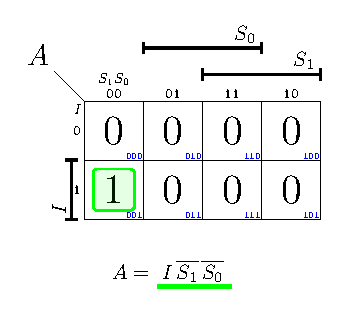
\includegraphics[width=4cm,trim={0.5cm 0.5cm  0.25cm 0.25cm},clip]{Ejercicio_3/Karnaugh/DEMUX/Salida_A.pdf}&
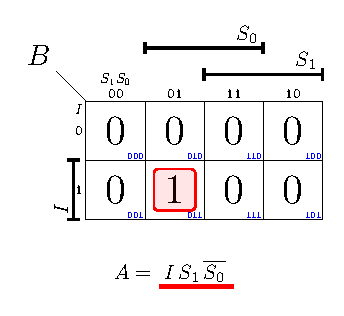
\includegraphics[width=4cm,trim={0.5cm 0.5cm  0.25cm 0.25cm},clip]{Ejercicio_3/Karnaugh/DEMUX/Salida_B.pdf}\\
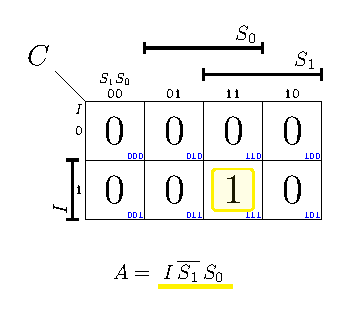
\includegraphics[width=4cm,trim={0.45cm 0.5cm  0.25cm 0.25cm},clip]{Ejercicio_3/Karnaugh/DEMUX/Salida_C.pdf}&
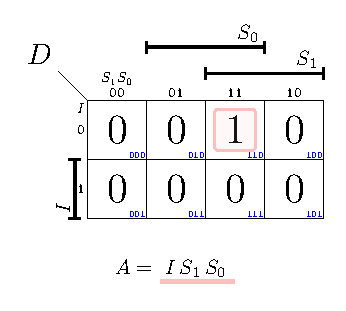
\includegraphics[width=4cm,trim={0.5cm 0.5cm  0.25cm 0.25cm},clip]{Ejercicio_3/Karnaugh/DEMUX/Salida_D.pdf}\\
\end{tabular}
    \caption{Mapas de Karnaugh de las salidas del Demultiplexor}
    \label{fig:Karnaughs_DEMUX} 
\end{figure}

Se procede a implementar el circuito hallado mediante los mapas:
\begin{figure}[H]
\centering
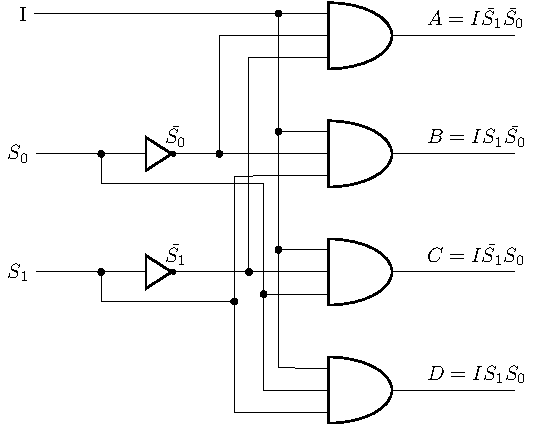
\includegraphics[width=6cm,height=4cm]{Ejercicio_3/Circuitos/Circuito_DEMUX.pdf}
\caption{Circuito Demultiplexor de 4 salidas}
\label{fig:Circuito_DEMUX}
\end{figure}
Respecto del diseño en verilog,

\subsection{Codificador de 4 entradas}
A continuación, se analiza la tabla de verdad de un codificador de 4 entradas:
\begin{table}[H]
	\begin{center}
		\begin{tabular}{|c|c|c|c||c|c|c|}
			\hline
			$A$ &	$B$ &	$C$ &	$D$ & $S_1$ & $S_0$& $E$ \\
			\hline

            1 & 0 & 0 & 0 & 0 & 0 & 0  \\
            \hline
  
            0 & 1 & 0 & 0 & 0 & 1 & 0 \\
            \hline
         
            0 & 0 & 1 & 0 & 1 & 0 & 0 \\
            \hline              
         
            0 & 0 & 0 & 1 & 1 & 1 & 0 \\
            \hline
            
            X & X & X & X & X & X & 1 \\
            \hline		
		\end{tabular}
		\caption{Tabla de verdad del Codificador}
	\end{center}
\end{table}
Cada salida distinta nos permitirá diagramar un mapa de Karnaugh propio. Se contempla el caso de un error cuando las entradas no sean propias a las de un codificador. Los mapas se presentan a continuación:

\begin{figure}[H]
   \centering
\begin{tabular}{ccc}
	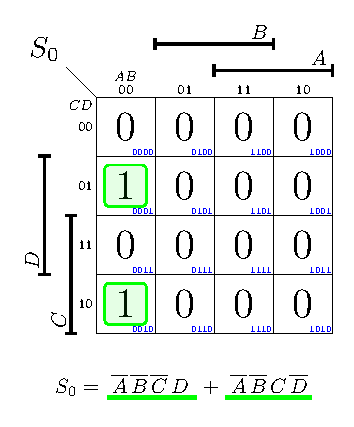
\includegraphics[width=4cm,trim={0.25cm 0.5cm  0.25cm 0.25cm},clip]{Ejercicio_3/Karnaugh/ENCODER/Salida_S_0.pdf}& \hspace{3ex} 
	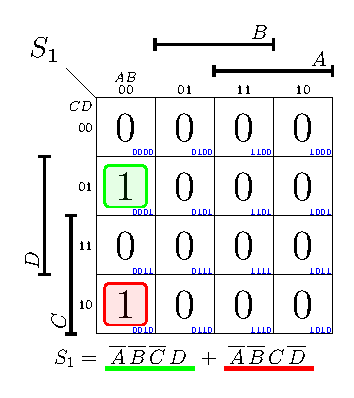
\includegraphics[width=4cm,trim={0.25cm 0.5cm  0.25cm 0.25cm},clip]{Ejercicio_3/Karnaugh/ENCODER/Salida_S_1.pdf}&
		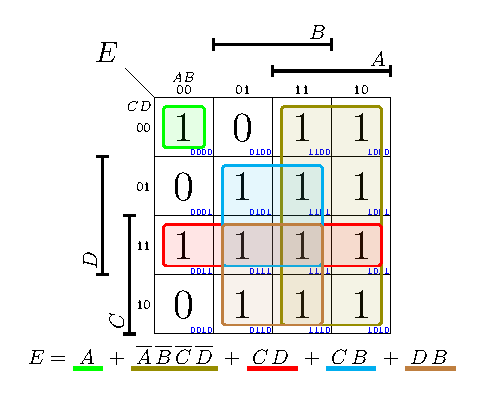
\includegraphics[width=5.5cm,trim={0.25cm 0.5cm  0.25cm 0.25cm},clip]{Ejercicio_3/Karnaugh/ENCODER/Salida_E.pdf}\\
	\end{tabular}
    \caption{Mapas de Karnaugh de las salidas del Codificador}
    \label{fig:Karnaughs_encoder} % 
\end{figure}
Por claridad, se coloca, por un lado, el circuito propio al codificador, y por otro, el utilizado para detectar un error. Sin embargo, los mismos podrían estar integrados. Los circuitos propuestos son los siguientes:

\begin{figure}[H]
\centering
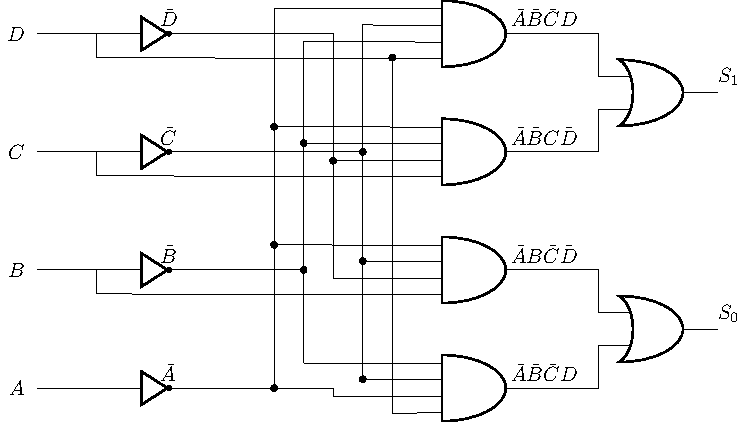
\includegraphics[width=7cm,height=4cm]{Ejercicio_3/Circuitos/Circuito_ENCODER.pdf}
\caption{Circuito Codificador de 4 entradas}
\label{fig:Circuito_ENCODER}
\end{figure}

\begin{figure}[H]
\centering
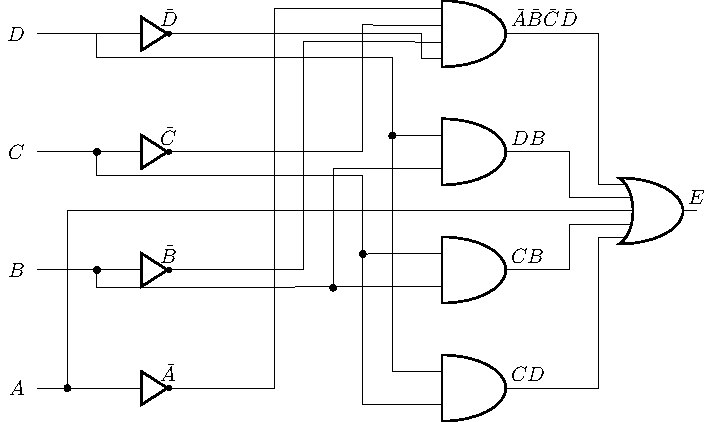
\includegraphics[width=7cm,height=4cm]{Ejercicio_3/Circuitos/Circuito_ENCODER_ERROR.pdf}
\caption{Circuito detector de error - Encoder}
\label{fig:Circuito_ENCODER_ERROR}
\end{figure}
